%        File: global_abstract.tex
%     Created: January 14, 2013
%      Author: Kathryn Huff

\documentclass{anstrans}
%%%%%%%%%%%%%%%%%%%%%%%%%%%%%%%%%%%
\title{ Cyclus Fuel Cycle Simulation Capabilities with the Cyder Disposal System Model}
\author{Kathryn D.~Huff}

%% uncomment these next five only if using anstrans
\institute{Argonne National Laboratory, 9700 S. Cass Ave., Lemont, IL 60439 \\
University of Wisconsin, 1500 Engineering Drive, Madison, WI 53706}
\email{katyhuff@gmail.com}
\usepackage{graphicx}
\usepackage{placeins}
\usepackage{glossaries}
\usepackage{xspace}
\usepackage{booktabs} % nice rules for tables
\usepackage{microtype} % if using PDF
\newcommand{\units}[1] {\:\text{#1}}%
\newcommand{\Cyclus}{\textsc{Cyclus}\xspace}%
\newcommand{\fluxJ}{\overrightarrow{J} }
\newcommand{\Cyder}{\textsc{Cyder}\xspace}
\newcommand{\SN}{S$_N$}%{S$_\text{N}$}%{$S_N$}%
\newacronym{MIT}{MIT}{the Massachusettes Institute of Technology}
\newacronym{UW}{UW}{University of Wisconsin}
\newacronym{US}{US}{United States}
\newacronym{IAEA}{IAEA}{International Atomic Energy Agency}
\newacronym{SNF}{SNF}{spent nuclear fuel}
\newacronym{HLW}{HLW}{high level waste}
\newacronym{FEHM}{FEHM}{Finite Element Heat and Mass Transfer}
\newacronym{DOE}{DOE}{Department of Energy}
\newacronym{GENIUSv2}{GENIUS}{Global Evaluation of Nuclear Infrastructure Utilization Scenarios, Version 2}
\newacronym{CNERG}{CNERG}{Computational Nuclear Engineering Research Group}
\newacronym{GDSM}{GDSM}{Generic Disposal System Model}
\newacronym{GDSE}{GDSE}{Generic Disposal Sytem Environment}
\newacronym{GPAM}{GPAM}{Generic Performance Asessment Model}
\newacronym{FEPs}{FEPs}{Features, Events, and Processes}
\newacronym{EBS}{EBS}{Engineered Barrier System}
\newacronym{EDZ}{EDZ}{Excavation Disturbed Zone}
\newacronym{YMR}{YMR}{Yucca Mountain Repository Site}
\newacronym{EPA}{EPA}{Environmental Protection Agency}
\newacronym{PEI}{PEI}{Peak Environmental Impact}
\newacronym{VISION}{VISION}{the Verifiable Fuel Cycle Simulation Model}
\newacronym{NUWASTE}{NUWASTE}{Nuclear Waste Assessment System for Technical Evaluation}
\newacronym{NWTRB}{NWTRB}{Nuclear Waste Technical Review Board}
\newacronym{OCRWM}{OCRWM}{Office of Civillian Radioactive Waste Management}
\newacronym{UFD}{UFD}{Used Fuel Disposition}
\newacronym{DYMOND}{DYMOND}{Dynamic Model of Nuclear Development }
\newacronym{DANESS}{DANESS}{Dynamic Analysis of Nuclear Energy System Strategies}
\newacronym{CAFCA}{CAFCA}{ Code for Advanced Fuel Cycles Assessment }
\newacronym{ORION}{ORION}{O..}
\newacronym{NFCSim}{NFCSim}{Nuclear Fuel Cycle Simulator}
\newacronym{COSI}{COSI}{Commelini-Sicard}
\newacronym{FCT}{FCT}{Fuel Cycle Technology}
\newacronym{SWF}{SWF}{Separations and Waste Forms}
\newacronym{FCO}{FCO}{Fuel Cycle Options}
\newacronym{RDD}{RD\&D}{Research Development and Design}
\newacronym{WIPP}{WIPP}{Waste Isolation Pilot Plant}
\newacronym{ANDRA}{ANDRA}{Agence Nationale pour la gestion des D\'echets RAdioactifs, the French National Agency for Radioactive Waste Management}
\newacronym{TSM}{TSM}{Total System Model}
\newacronym{LANL}{LANL}{Los Alamos National Laboratory}
\newacronym{INL}{INL}{Idaho National Laboratory}
\newacronym{ANL}{ANL}{Argonne National Laboratory}
\newacronym{SNL}{SNL}{Sandia National Laboratory}
\newacronym{LBNL}{LBNL}{Lawrence Berkeley National Laboratory}
\newacronym{LLNL}{LLNL}{Lawrence Livermore National Laboratory}
\newacronym{NAGRA}{NAGRA}{National Cooperative for the Disposal of Radioactive Waste}
\newacronym{CUBIT}{CUBIT}{CUBIT Geometry and Mesh Generation Toolkit}
\newacronym{CSNF}{CSNF}{Commercial Spent Nuclear Fuel}
\newacronym{DSNF}{DSNF}{DOE Spent Nuclear Fuel}
\newacronym{MTHM}{MTHM}{Metric Ton of Heavy Metal}
\newacronym{HTGR}{HTGR}{High Temperature Gas Reactor}
\newacronym{TRISO}{TRISO}{Tristructural Isotropic}
\newacronym{MA}{MA}{Minor Actinide}
\newacronym{STC}{STC}{Specific Temperature Change}
\newacronym{CEA}{CEA}{Commissariat a l'Energie Atomique et aux Energies Alternatives}
\newacronym{SKB}{SKB}{Svensk Karnbranslehantering AB}
\newacronym{SINDAG}{SINDA{\textbackslash}G}{Systems Improved Numerical Differencing Analyzer $\backslash$ Gaski}
%\newacronym{<++>}{<++>}{<++>}

\makeglossaries


\date{}
%%%%%%%%%%%%%%%%%%%%%%%%%%%%%%%%%%%
\begin{document}
%%%%%%%%%%%%%%%%%%%%%%%%%%%%%%%%%%%%%%%%%%%%%%%%%%%%%%%%%%%%%%%%%%%%%%%%%%%%%%%%
\textit{An algorithm and supporting database for rapid thermal repository 
loading calculation was implemented in }\Cyder.\textit{ This algorithm employs a 
\gls{STC} 
method \cite{radel_effect_2007, radel_repository_2007} and has resulted from 
combining detailed spent nuclear fuel composition data \cite{carter_fuel_2011} 
with a detailed thermal repository performance analysis tool from \gls{LLNL}, 
\gls{ANL}, and the \gls{UFD} campaign \cite{greenberg_application_2012}. By 
abstraction of 
and benchmarking against these detailed thermal models, \Cyder captures the 
dominant physics of thermal phenomena affecting repository capacity in various 
geologic media and as a function of spent fuel composition.

Abstraction based on detailed computational thermal repository performance 
calculations with the \gls{LLNL} semi-analytic model has resulted in 
implementation 
of the \gls{STC} estimation algorithm and a supporting reference dataset.  This 
method is capable of rapid estimation of temperature increase near emplacement 
tunnels as a function of waste composition, limiting radius, $r_{lim}$, waste 
package spacing, $S$, near field thermal conductivity, $K_{th}$, and near field 
thermal diffusivity, $\alpha_{th}$.
}


The results here provide an overview of the relative importance of thermal
parameters that that affect the repository capacity of simplified generic
disposal concept in various geologic media where conduction is the dominant
heat transfer mode. The applicability of this sensitivity analysis is thus
restricted to enclosed, backfilled concepts.  

\subsection{Parametric Domain}

Sensitivity analyses were conducted which span the parametric range of values 
generated by the reference specific temperature change database and described 
in Table \ref{tab:thermal_cases}.  

These values were selected to provide detail in the near field and at values of
$\alpha_{th}$ and $K_{th}$ in the three host media under consideration in this
work.

\subsection{Approach}

% used existing gdsms 
This analysis utilized the \gls{LLNL} semi-analytic MathCAD model utilized to 
derive supporting data and to validate behaviro within the \Cyder STC model. It 
performs detailed calculations of the conductive thermal transport in a generic 
repository concept with a gridded layout.  

It relies on the thermal diffusivity, $\alpha_{th}$ and conductivity $K_{th}$ of 
the material as well as the waste package spacing, $S$, and thermally limiting 
radius, $r_{lim}$. Finally, it relies on the \gls{STC} data calculated with the 
semi-analytic model based on the decay heat profiles of the emplace wastes, $Q$. 
The essential decay heat profiles, $Q$, were retrieved from a \gls{UFD} database 
provided by Carter et al. \cite{carter_fuel_2011}.



\section{\textsc{Cyder} Repository Modeling Paradigm}

The \Cyder disposal system simulator architecture is intended to modularly permit 
exchange of disposal system Component models (e.g., detailed nuclide transport 
model vs. less detailed) and data (e.g., exchange clay for granite geologic 
data) and accept arbitrary waste stream isotopic compositions.  
Finally, in order to participate in a \Cyclus simulation as a facility model, \Cyder must 
make requests for spent material up to its capacity. Determination of the 
repository capacity for various types of spent fuel commodities comprises the 
interfacing functionality of the repository model.

\subsection{Waste Stream Acceptance}

The disposal system simulator must accept arbitrary spent fuel and high level waste 
streams. A waste stream is a material data object resulting from the \Cyclus 
simulated fuel cycle.  As radionuclides are gained, lost, and transmuted within 
the spent fuel object, a history of its isotopic composition is recorded.  It 
arrives at the repository and is emplaced if it obeys all repository capacity 
limits. 

For waste streams that vary from each other in composition, the thermal 
capacity of the repository to receive that waste stream must therefore be 
recalculated.  Since disposable material in most simulations of interest will 
be of variable composition and therefore heterogeneous in heat production 
capability, the disposal system simulator will repeatedly need to recalculate its own 
capacity as new materials are offered.  

\subsection{Waste Stream Conditioning}

Waste conditioning is the process of packing a waste stream into an appropriate 
waste form. As \Cyclus lacks a conditioning facility, the \Cyder repository 
fulfills this need as a part of the repository behavior. As a waste stream is 
accepted into the repository, it is associated with a waste form according 
to its commodity name. This pairing is input by the user during simulation 
setup when a number of waste form Component configurations are specified and 
associated with allowed waste stream commodities. It is according to these 
pairings that \Cyder loads discrete waste forms with discrete waste 
stream contaminant vectors as depicted in Figure \ref{fig:ws_conditioning}.

\begin{figure}[htbp!]
\begin{center}
\def\svgwidth{.5\columnwidth}
\input{./paradigm/ws_conditioning.eps_tex}
\end{center}
\caption[Waste stream conditioning in \Cyder.]{Waste streams are accepted and 
conditioned into the appropriate waste form according to user-specified 
pairings between commodities and waste forms.}
\label{fig:ws_conditioning}
\end{figure}

\subsection{Waste Form Packaging}

Waste packaging is the process of placing one or many waste forms into a 
containment package (typcially metallic). Once the waste stream has been 
conditioned into a waste form, that waste form Component is loaded into a waste 
package Component, also according to allowed pairs dictated by the user, as 
depicted in Figure \ref{fig:wf_packaging}.

\begin{figure}[htbp!]
\begin{center}
\def\svgwidth{.5\columnwidth}
\input{./paradigm/wf_packaging.eps_tex}
\end{center}
\caption[Waste packaging in \Cyder.]{Waste forms are loaded into the 
appropriate waste package according to user-specified pairings between forms 
and packages.}
\label{fig:wf_packaging}
\end{figure}


\subsection{Package Emplacement}

Finally, the waste package is emplaced in a buffer component, which 
contains many other waste packages, spaced evenly in a grid. The grid is 
defined by the user input and depends on repository depth, $\Delta z$, waste 
package spacing, $\Delta x$, and tunnel spacing, $\Delta y$ as in Figure 
\ref{fig:repo_layout}.

\begin{figure}[htbp!]
\begin{center}
\def\svgwidth{.5\columnwidth}
\input{./paradigm/repo_layout.eps_tex}
\end{center}
\caption[The gridded \Cyder repository emplacement geometry.]{The \Cyder 
repository emplacement geometry allows generic representation of all semi-regular 
two dimensional gridded layouts.}
\label{fig:repo_layout}
\end{figure}

\subsection{Nested Components}

The fundamental unit of information in the disposal system simulator is radionuclide 
contaminant presence at each stage of containment.  The disposal system simulator, in 
this way, is fundamentally a tool to determine thermal and contaminant 
transport evolution as a result of an arbitrary waste stream. The disposal 
system simulator in this work conducts this calculation by  treating each containment 
Component as a nested volume in a release chain. 

Each Component is defined by a Geometry, some Material Data, a ThermalModel, 
and a NuclideModel. It is also defined by the Parent Component which contains 
it and the daughter components which it contains. An emplaced waste package 
Component, for example, possesses a pointer to the buffer that surrounds it, 
its Parent Component. It also possesses a list of pointers to the waste form or 
waste forms within it, its daughter components. 

\subsubsection{Component Geometry}

Each Component of the repository system (i.e. waste form, waste package, buffer, 
and geologic medium) is modeled as a discrete control volume. Each control 
volume performs its own mass balance at each time step and assesses its own 
internal  heat transfer and degradation phenomena utilizing boundary condition 
information provided by adjacent nested Components. This control volume is 
defined by the Component Geomtry, a class which keeps track of the inner and 
outer radii, length, and centroid coordinates of the (assumed cylindrical) 
volume.

\subsubsection{Component Material Data}

Each Component of the repository system possesses a notion of the material that 
it is made of. Supporting thermal and hydrologic data for canonical engineered 
barrier and geologic media is provided with the code in the 
mat\_data.sqlite SQLite database.

Each table in the database holds data related to one of a canonical set of 
engineered barrier and geologic medium materials (e.g. clay, glass, etc.).  
The columns of that table hold data required to support all \Cyder models. 
Thermal diffusivity and thermal conductivity comprise the thermal data in the 
table for each material. The hydrologic and chemical data in the database has 
one table for each material. Each table contains relative diffusivity 
coefficients, solubility limits, and sorption parameters for each element.  

\subsubsection{Component ThermalModel}

Each Component possesses a thermal transport model that determines the 
temperature inside the Component over time. This allows limitations within any 
barrier at any limiting radius to control the limiting thermal response within 
the \Cyder repository simulator. 

\subsubsection{Component NuclideModel}

Each Component possesses a radionuclide contaminant transport model that 
determines the contaminant transport inside the Component over time. The 
choices available for this NuclideModel range in fidelity but emphasize the 
distinction between dominant transport modes (advective or disperive) in 
various geologic media as well as dominant retarding geochemistry for specific 
isotopes (sorption and solubility limitation).

\subsubsection{Implicit Timestepping}

Each Component passes some information radially outward to the nested 
Component immediately containing it and some information radially 
inward to the nested Component it contains. 


In the case of radionuclide transport, for example, each Component model
requires information about the radionuclides released from the Component it
immediately contains.  Thus, nuclide release information is passed radially
outward from the waste stream sequentially through each containment layer to
the geosphere. However, the solutions within each Component often rely on the
external boundary conditions of that Component.  Thus, the \Cyder model uses an
implicit timestepping method to arrive at the future state of each Component,
radially outward, as a function of both the past state and the current state. 

That is, in Component j, some Component in a nested series, the mass flux 
entering the Component at time $t_n$ is found from the initial state of the cell 
at time $t_n$, the inner boundary 
condition at time $t_n$ and the outer boundary condition at $t_{n-1}$.  

\begin{align}
  \dot{m}_{ij}^n &= f( m_j(t_{n-1}) , BC_i(t_n) , BC_j(t_{n-1}) . . . ) \nonumber\\
  \intertext{where}
  m_{ij}(t_n) &= \mbox{ contaminant mass flux from component i to j }[kg/timestep]\nonumber\\
  BC_i(t_n)  &= \mbox{ inner conditions at }r_i\mbox{, and time }t_n \nonumber \\
  BC_j(t_{n-1})  &= \mbox{ outer conditions at }r_j\mbox{, and time }t_{n-1} \nonumber\\
  f &= \mbox{ functional form of contaminant transport into j. }\nonumber
\end{align}

Once the mass flux into the component is found, the mass is removed from the 
inner cell, updating its state in preparation for the next time step.

\begin{align}
  m_i^\dagger(t_n)  &= m_i(t_n)  - m_{ij}(t_n) 
  \intertext{where}
  m_i^\dagger(t_n)  &= \mbox{ updated mass in component i }[kg]
\end{align}

In this way, the contained mass in the component is described as
\begin{align}
  m_j(t_n)  &= m_j(t_{n-1})  + \dot{m}_j(t_n) . \nonumber
\end{align}

Resulting concentration profiles across the component can then be calculated 
and one can solve, numerically, for the outer boundary condition at $t_n$ 

\begin{align}
  BC_j(t_n) &= g\left( m_j(t_n) , C_j(t_n) \right)\nonumber\\
  g &= \mbox{functional form of contaminant transport across j}\nonumber
\end{align}

This boundary condition can, in turn, be used by the component external to it, $k$ as the $t_n$ 
inner boundary condition of its own solution and so on.




\section{Thermal Transport Analysis}

For dynamic thermal capacity analysis in Cyder, a transient model utilizes a 
linear approximation of heat based capacity quickly for each 
arbitrary waste stream offered to the repository. This relies on a thermal reference database of repository heat 
evolution curves covering the thermal coefficient range of the main geologies of 
interest and over a range of realistic waste package spacings. 
\subsection{Supporting Thermal Response Dataset}
To support this calculation in \Cyder , a reference data set of temperature change 
curves was calculated. Repeated runs of a detailed analytic model over the range of values in Table 
\ref{tab:thermal_cases} determined \gls{STC} values over a range of thermal 
heat limit radii, $r_{lim}$, thermal diffusivity values, $\alpha_{th}$,
thermal conductivity values, $K_{th}$ and waste package spacings, $S$. Linear 
interpolation across the discrete parameter space provides a simple thermal 
reference dataset for use in \Cyder .

\begin{table}[ht!]
\centering
\footnotesize{
\begin{tabular}{|l|l|l|r|}
\multicolumn{4}{c}{\textbf{Thermal Cases}}\\
\hline
\textbf{Parameter} & \textbf{Symbol} & \textbf{Units} & \textbf{Value Range} \\
\hline
Diffusivity & $\alpha_{th}$ & $[m^2\cdot s^{-1}]$ & $1.0\times10^{-7}$\\
 & & & $2.0\times10^{-7}$\\
 & & & $3.0\times10^{-7}$\\
 & & & $4.0\times10^{-7}$\\
 & & & $5.0\times10^{-7}$\\
 & & & $6.0\times10^{-7}$\\
 & & & $7.0\times10^{-7}$\\
 & & & $8.0\times10^{-7}$\\
 & & & $9.0\times10^{-7}$\\
 & & & $1.0\times10^{-6}$\\
 & & & $2.0\times10^{-6}$\\
 & & & $3.0\times10^{-6}$\\
\hline
Conductivity & $K_{th}$     & $[W\cdot m^{-1} \cdot K^{-1}]$  & $0.1, 0.5, 1, 1.5, 2, 2.5, 3, 3.5, 4, 4.5 $ \\
\hline
Spacing & $S$ & $[m]$ & 2, 5, 10, 15, 20, 25, 50 \\
\hline
Radius & $r_{lim}$ & $[m]$ & 0.1, 0.25, 0.5, 1, 2, 5 \\
\hline
Isotope & $i$ & $[-]$ & $^{241,243}Am,$  \\
        & & & $^{242,243,244,245,246}Cm,$  \\
        & & & $^{238,240,241,242}Pu$  \\
        & & & $^{134,135,137}Cs$  \\
        & & & $^{90}Sr$  \\
\hline
\end{tabular}
\caption{A thermal reference dataset of \gls{STC} values as a function of each of these parameters was generated by repeated parameterized runs of the LLNL 
MathCAD model\cite{greenberg_application_2012, greenberg_investigations_2012}.}
\label{tab:thermal_cases}
}
\end{table}



The analytic model used to populate the reference dataset was created at 
\gls{LLNL} for the \gls{UFD} campaign. In this tool, heat limited thermal 
response is calculated analytically for each geology, for many waste package 
loading densities, and for many fuel cycle options \cite{hardin_generic_2011, 
greenberg_investigations_2012, greenberg_application_2012}. It employs an 
analytic model from Carslaw and Jaeger and is implemented in MathCAD 
\cite{carslaw_conduction_1959, ptc_mathcad_2010}.  The integral solver in the 
MathCAD toolset is the primary calculation engine for the analytic MathCAD 
thermal model, which relies on superposition of point, finite-line, and line 
source integral solutions.  

%The transient state of the temperature at the calculation radius is found with a convolution of the transient far field solution with the steady state near field solution.  The process is then iterated with a one year resolution in order to arrive at a temperature evolution over the lifetime of the repository. 
%
%In a two dimensional grid of waste packages, the central package is represented by the finite line solution

Figure \ref{fig:CmScaling} demonstrates the scaling of an STC curve according to 
equation \eqref{STC} to represent the heat from $25.9g$ of initial $^{242}Cm$ using 
the reference data set. 

\begin{figure}[h!]
\begin{center}
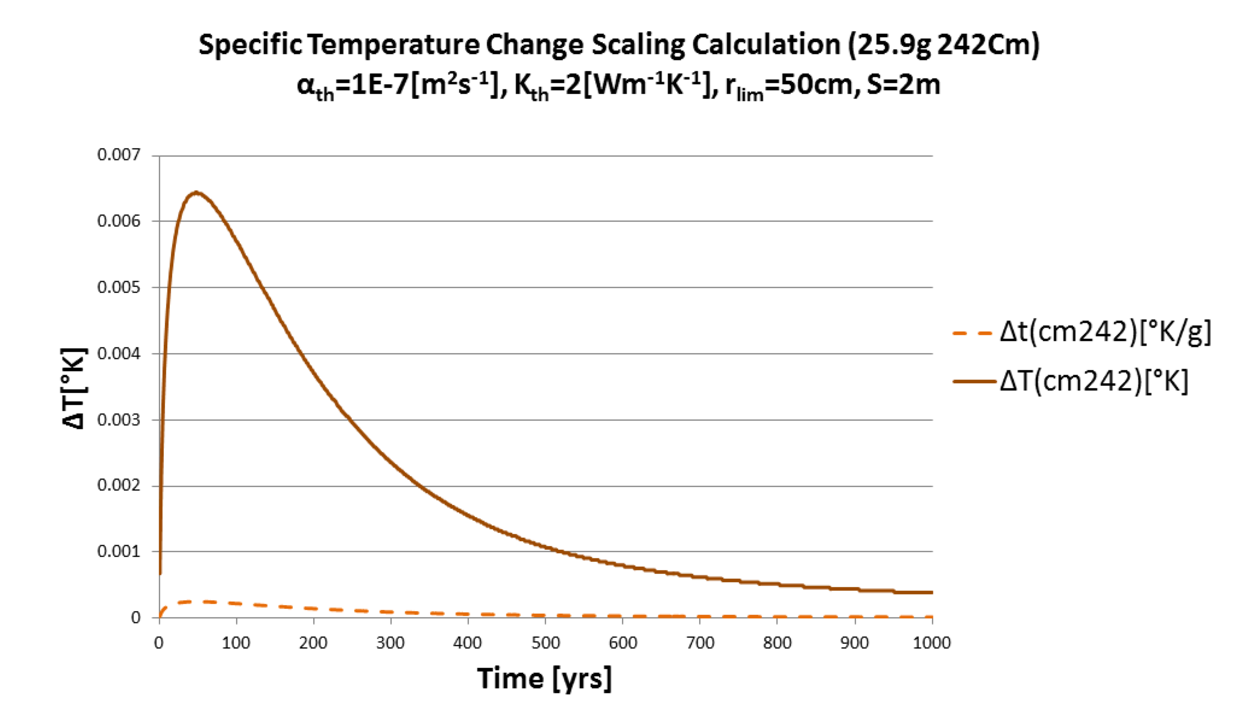
\includegraphics[width=\columnwidth]{./thermal_models/CmScaling.eps}
\end{center}
\caption{As a demonstration of the calculation procedure, the temperature change 
  curve for one initial gram of $^{242}Cm$ and is scaled to represent $25.9g$, 
  approximately the $^{242}Cm$ inventory per MTHM in 51GWd burnup UOX PWR fuel. }
\label{fig:CmScaling}
\end{figure}


The supporting database was limited to some primary heat contributing isotopes 
present in traditional spent nuclear fuel, $H$, 
such that the superposition in equation \eqref{superposition} becomes 

\begin{align}
\Delta T (r_{lim},S,K_{th},\alpha_{th})&\sim \sum_{i\in H} m_i \Delta t_i(r_{lim},S,K_{th},\alpha_{th})
\label{superposition_approx}
\intertext{where}
H &= \mbox{ set of high heat isotopes }[-]\nonumber\\
S &= \mbox{ uniform waste package spacing } [m]\nonumber\\
K_{th} &= \mbox{ thermal conductivity } [W\cdot m^{-1}\cdot K^{-1}]\nonumber\\
\alpha_{th} &= \mbox{ thermal diffusivity } [m^2\cdot s^{-1}]\nonumber\\
\end{align}

The use of this superposition is demonstrated in Figure 
\ref{fig:CmSuperposition}.

\begin{figure}[ht!]
\begin{center}
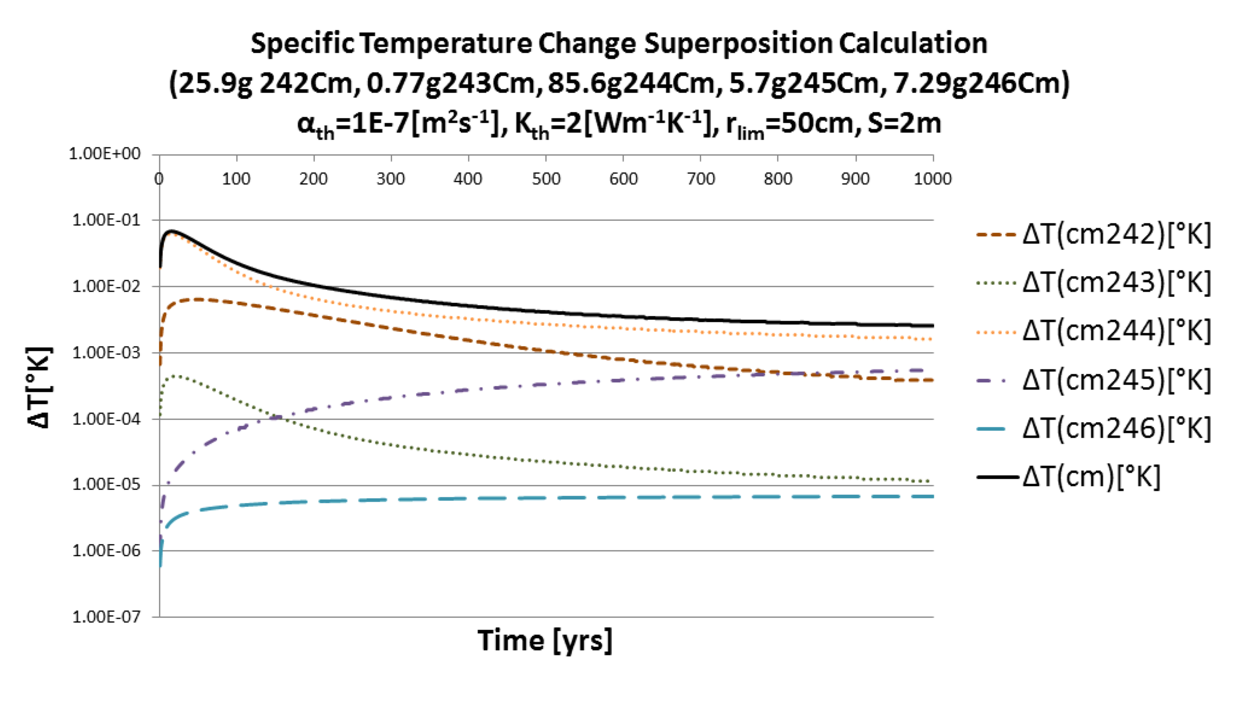
\includegraphics[width=\columnwidth]{./thermal_models/CmSuperposition.eps}
\end{center}
\caption{As a demonstration of the calculation procedure, scaled temperature change 
  curves for five curium isotopes are superimposed to achieve a total temperature 
change (note log scale).}
\label{fig:CmSuperposition}
\end{figure}

%\begin{align}
%  T_{line}(t,x,y,z) &= \frac{1}{8\pi K_{th}} 
%  \bigintsss_0^t\!\frac{q_L(t')}{t-t'}e^{ \frac{-\left(x^2 + z^2\right)}{4\alpha 
%  (t-t')} }\nonumber\\ &\cdot\left[ \erf{\left[ \frac{1}{2} \frac{\left( y + 
%  \frac{L}{2} \right)}{\sqrt{\alpha(t-t')}}  \right]} - \erf{\left[ \frac{1}{2} 
%  \frac{\left( y - \frac{L}{2} \right)}{\sqrt{\alpha(t-t')}}  \right]} 
%  \right]\,\mathrm{dt'},
%  \label{line}
%  \intertext{adjacent packages within the central tunnel are represented by the 
%  point source solution }
%  T_{point}(t,r) &= 
%  \frac{1}{8K_{th}\sqrt{\alpha}\pi^{\frac{3}{2}}}\bigintsss_0^{-t}\!\frac{q(t')}{(t-t')^{\frac{3}{2}}}e^{\frac{-r^2}{4\alpha(t-t')}}\,\mathrm{dt'},
%  \label{point}
%  \intertext{and adjacent disposal tunnels are represented by infinite line 
%  source solutions}
%  T_{\infty line}(t,x,z) &= \frac{1}{4\pi K_{th}} 
%  \bigintsss_0^t\!\frac{q_L(t')}{t-t'}e^{ \frac{-\left(x^2 + z^2\right)}{4\alpha 
%  (t-t')} }
%  \intertext{in infinite homogeneous media, where}
%  \label{infline}
%  \alpha &= ~~\mbox{thermal diffusivity } [m^2\cdot s^{-1}]\nonumber\\
%  q(t) &= ~~\mbox{point heat source} [W]\nonumber\\
%  \intertext{and}
%  q_L(t) &= ~~\mbox{linear heat source} [W\cdot m^{-1}]\nonumber
%\end{align}
%Superimposed point and line source solutions allow for a notion of the 
%repository layout to be modeled in the host rock.

\subsection{Thermal Transport Validation}\label{sec:thermal_benchmarks}

The results here provide an overview of the relative importance of thermal
parameters that that affect the repository capacity of simplified generic
disposal concept in various geologic media where conduction is the dominant
heat transfer mode. The applicability of this sensitivity analysis is thus
restricted to enclosed, backfilled concepts.  

\subsection{Parametric Domain}

Sensitivity analyses were conducted which span the parametric range of values 
generated by the reference specific temperature change database and described 
in Table \ref{tab:thermal_cases}.  

These values were selected to provide detail in the near field and at values of
$\alpha_{th}$ and $K_{th}$ in the three host media under consideration in this
work.

\subsection{Approach}

% used existing gdsms 
This analysis utilized the \gls{LLNL} semi-analytic MathCAD model utilized to 
derive supporting data and to validate behaviro within the \Cyder STC model. It 
performs detailed calculations of the conductive thermal transport in a generic 
repository concept with a gridded layout.  

It relies on the thermal diffusivity, $\alpha_{th}$ and conductivity $K_{th}$ of 
the material as well as the waste package spacing, $S$, and thermally limiting 
radius, $r_{lim}$. Finally, it relies on the \gls{STC} data calculated with the 
semi-analytic model based on the decay heat profiles of the emplace wastes, $Q$. 
The essential decay heat profiles, $Q$, were retrieved from a \gls{UFD} database 
provided by Carter et al. \cite{carter_fuel_2011}.



%\input{./thermal_demonstration/isotopics/isotopics}


\begin{frame}[ctb!]
\frametitle{LLNL Model Thermal Conductivity Sensitivity}

\begin{figure}[htbp!]
\begin{center}
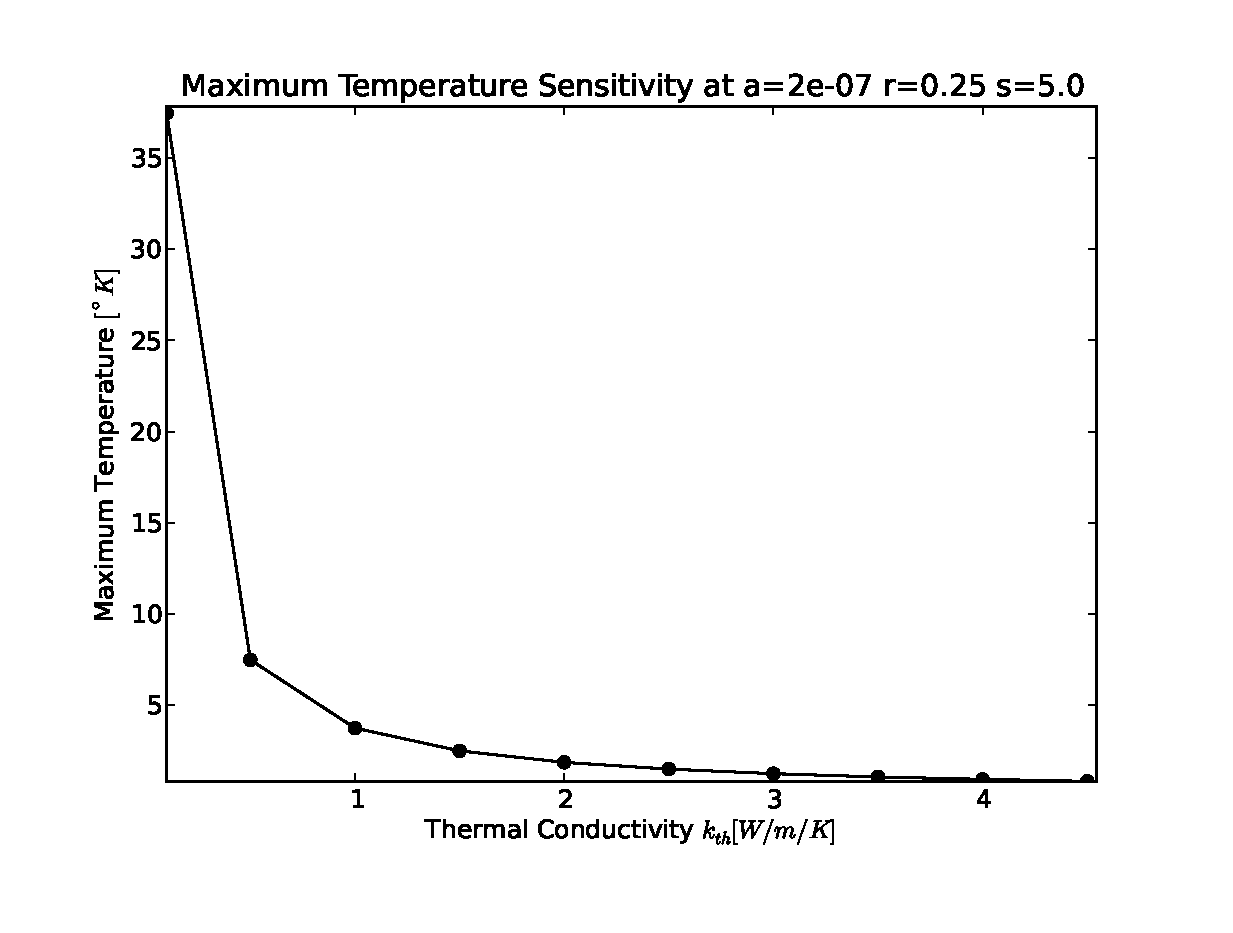
\includegraphics[height=0.7\textheight]{./thermal_demonstration/conductivity/conductivity.eps}
\end{center}
\caption[$K_{th}$ Sensitivity in LLNL Model]{Increased thermal conductivity decreases thermal energy deposition 
(here represented by STC) in the near field (here $r_{calc} = 0.5m$).}
\label{fig:Cm242Kth_alpha_low}
\end{figure}

\end{frame}


\begin{frame}[ctb!]
\frametitle{Cyder Thermal Conductivity Sensitivity}
\begin{figure}[htbp!]
\begin{center}
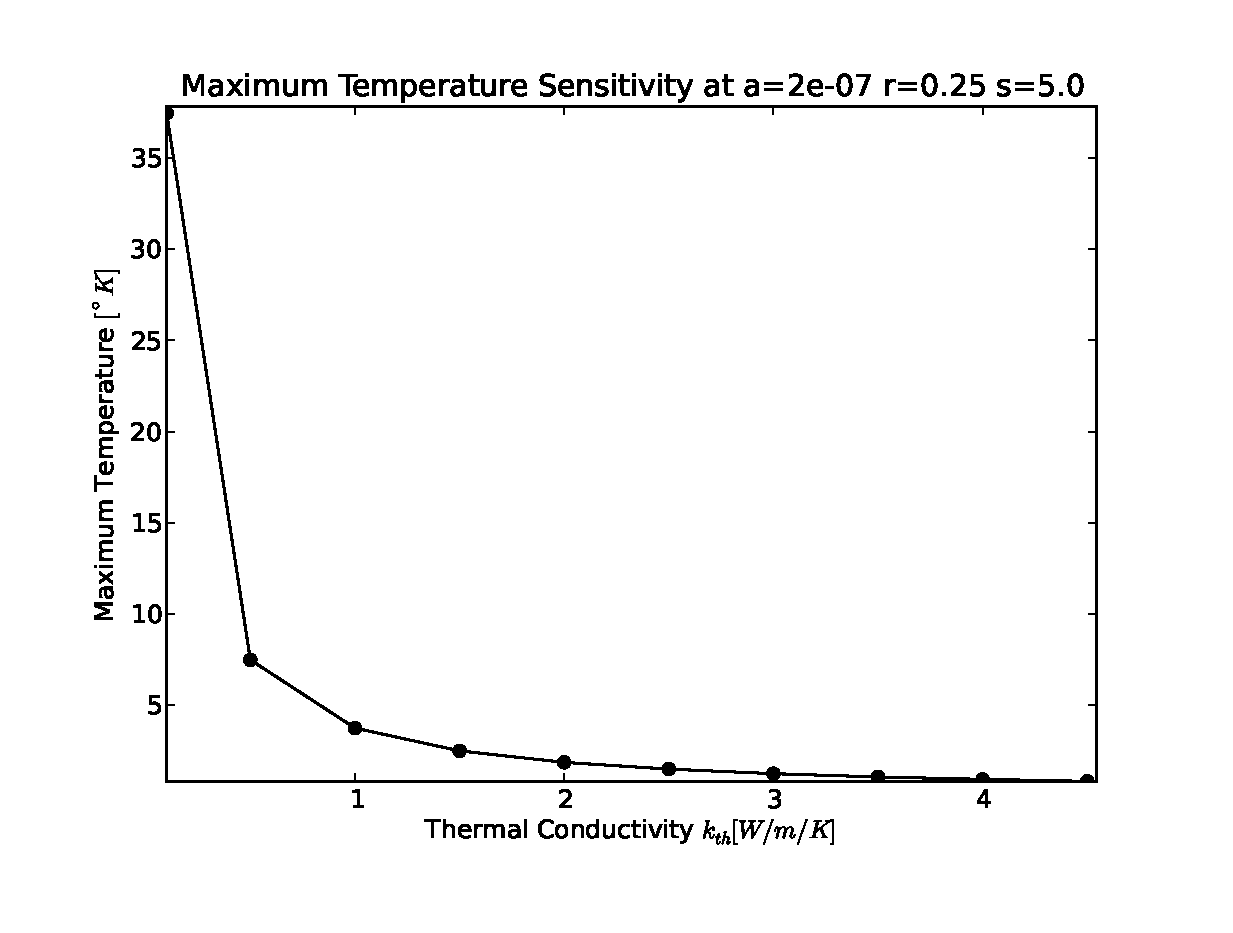
\includegraphics[height=0.7\textheight]{./thermal_demonstration/conductivity/conductivity.eps}
\end{center}
\caption[$K_{th}$ Sensitivity in Cyder]
{Cyder results agree with those of the LLNL model. Increased $K_{th}$ decreases 
thermal energy deposition at the limiting radius. The above example thermal 
profile results from 10kg of $^{242}Cm$, $\alpha_{th}=$, $s=$, and $r_{lim}=$.}
\label{fig:kr}
\end{figure}
\end{frame}

%\begin{frame}[ctb!]
%\frametitle{Cyder Thermal Conductivity and Limiting Radius Sensitivity}
%\begin{figure}[htbp!]
%\begin{center}
%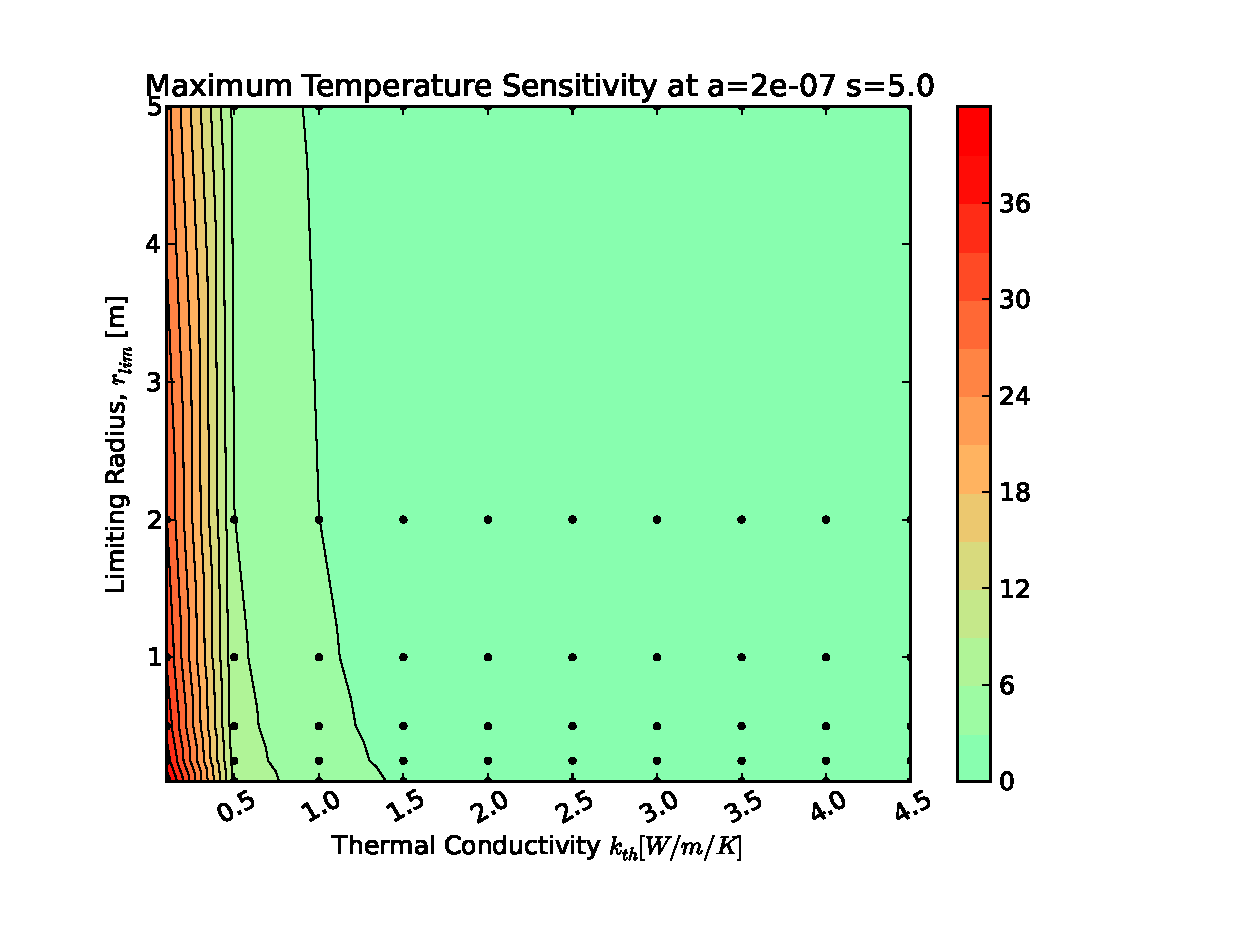
\includegraphics[height=0.7\textheight]{./thermal_demonstration/conductivity/kr.eps}
%\end{center}
%\caption[$K_{th}$ vs. $r_{lim}$ Sensitivity in Cyder]
%{Cyder results agree with 
%those of the LLNL model. The importance of the limiting radius decreases with 
%increased $K_{th}$. The above example thermal profile results from 10kg of 
%$^{242}Cm$}
%\label{fig:kr}
%\end{figure}
%\end{frame}


%\begin{frame}[ctb!]
%\frametitle{Cyder Thermal Conductivity and Limiting Radius Sensitivity}
%\begin{figure}[htbp!]
%\begin{center}
%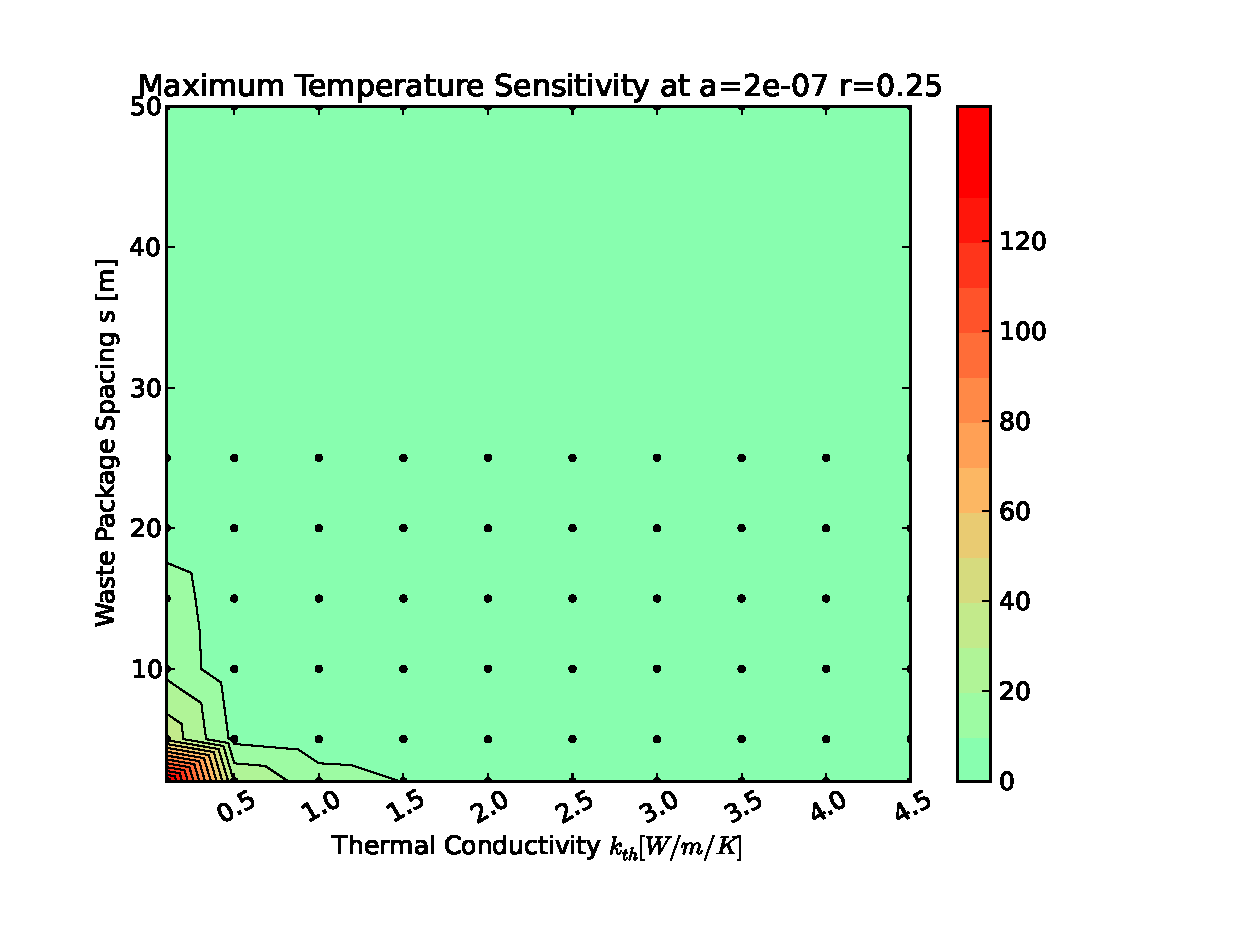
\includegraphics[height=0.7\textheight]{./thermal_demonstration/conductivity/ks.eps}
%\end{center}
%\caption[$K_{th}$ vs. Waste Package Spacing Sensitivity in Cyder]{Cyder results agree with 
%those of the LLNL model. The importance of the limiting radius decreases with 
%increased $K_{th}$. The above example thermal profile results from 10kg of 
%$^{242}Cm$}
%\label{fig:ks}
%\end{figure}
%\end{frame}


\begin{frame}[ctb!]
\frametitle{LLNL Model Thermal Diffusivity Sensitivity}
\begin{figure}[htbp!]
\begin{center}
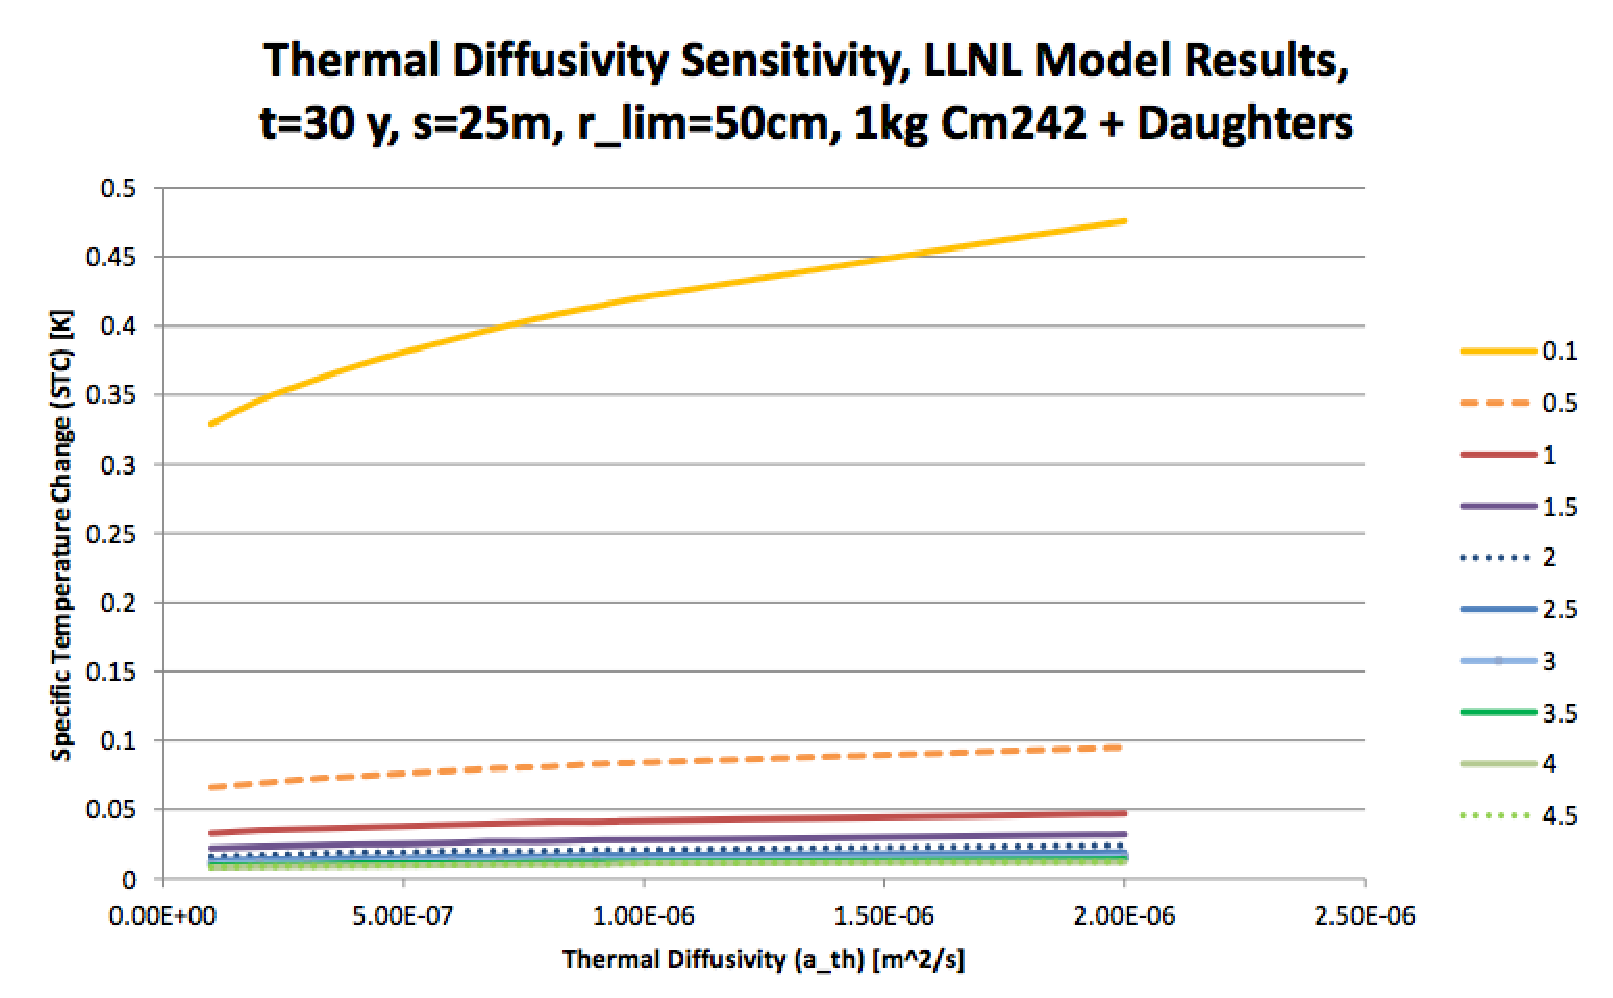
\includegraphics[height=0.7\textheight]{./thermal_demonstration/diffusivity/diffusivity.eps}
\end{center}
\caption[$K_{th}$ Sensitivity to $\alpha_{th}$]{Increased thermal 
diffusivity decreases temperature change (here represented by STC) at the 
limiting radius (here $r_{calc} = 0.5m$).}
\label{fig:Cm242alpha_kth_low}
\end{figure}
\end{frame}

\begin{frame}[ctb!]
\frametitle{Cyder Thermal Diffusivity Sensitivity}
\begin{figure}[htbp!]
\begin{center}
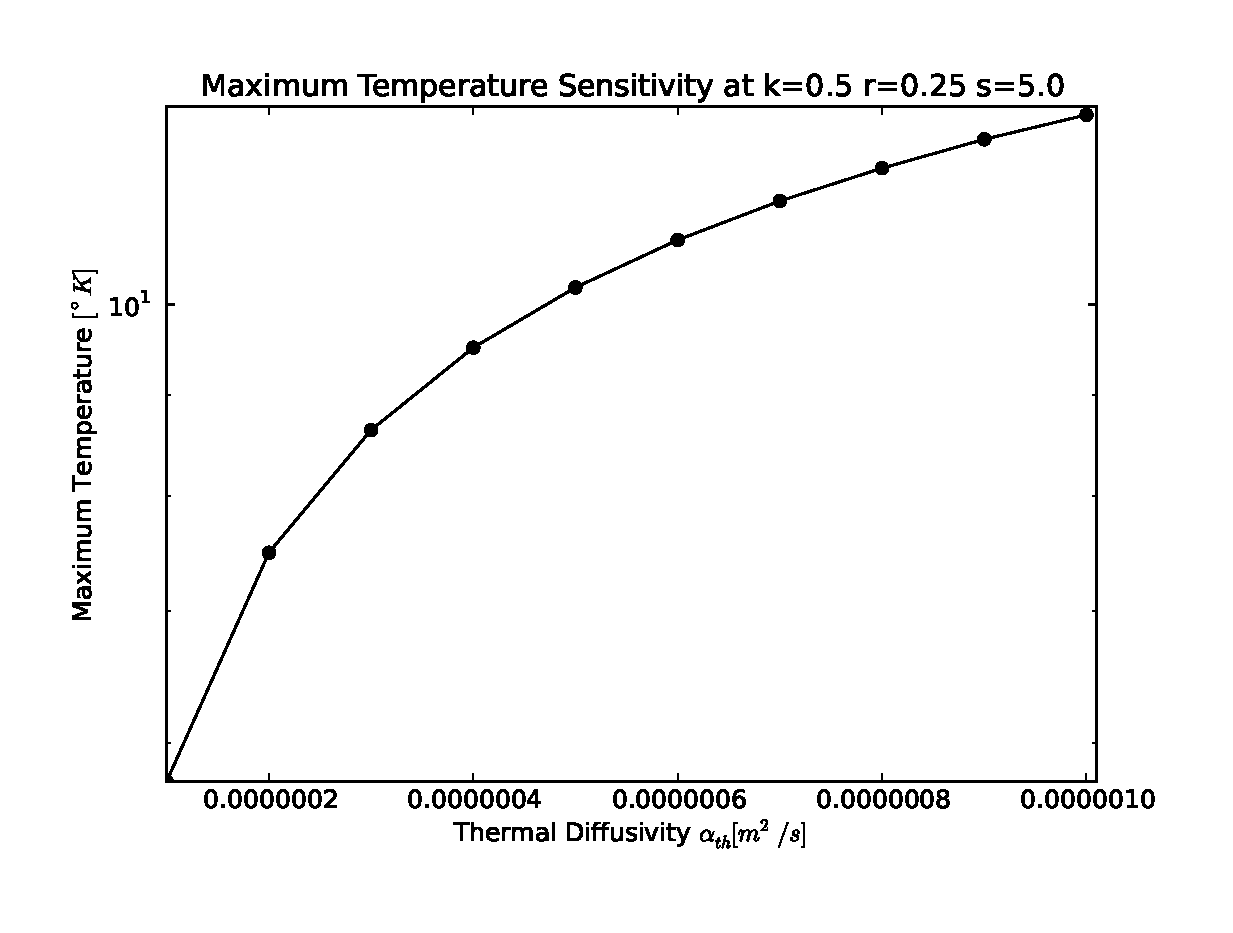
\includegraphics[height=0.7\textheight]{./thermal_demonstration/diffusivity/diffusivity_cyder.eps}
\caption[$\alpha_{th}$ Sensitivity in Cyder]{Cyder trends agree with those of 
the LLNL model, in which increased thermal diffusivity results in reduced 
temperature change at the limiting radius. The above example thermal profile 
results from 10kg of $^{242}Cm$.} 
\label{fig:ar}
\end{center}
\end{figure}
\end{frame}

%\begin{frame}[ctb!]
%\frametitle{Cyder Thermal Diffusivity and Conductivity Sensitivity}
%\begin{figure}[htbp!]
%\begin{center}
%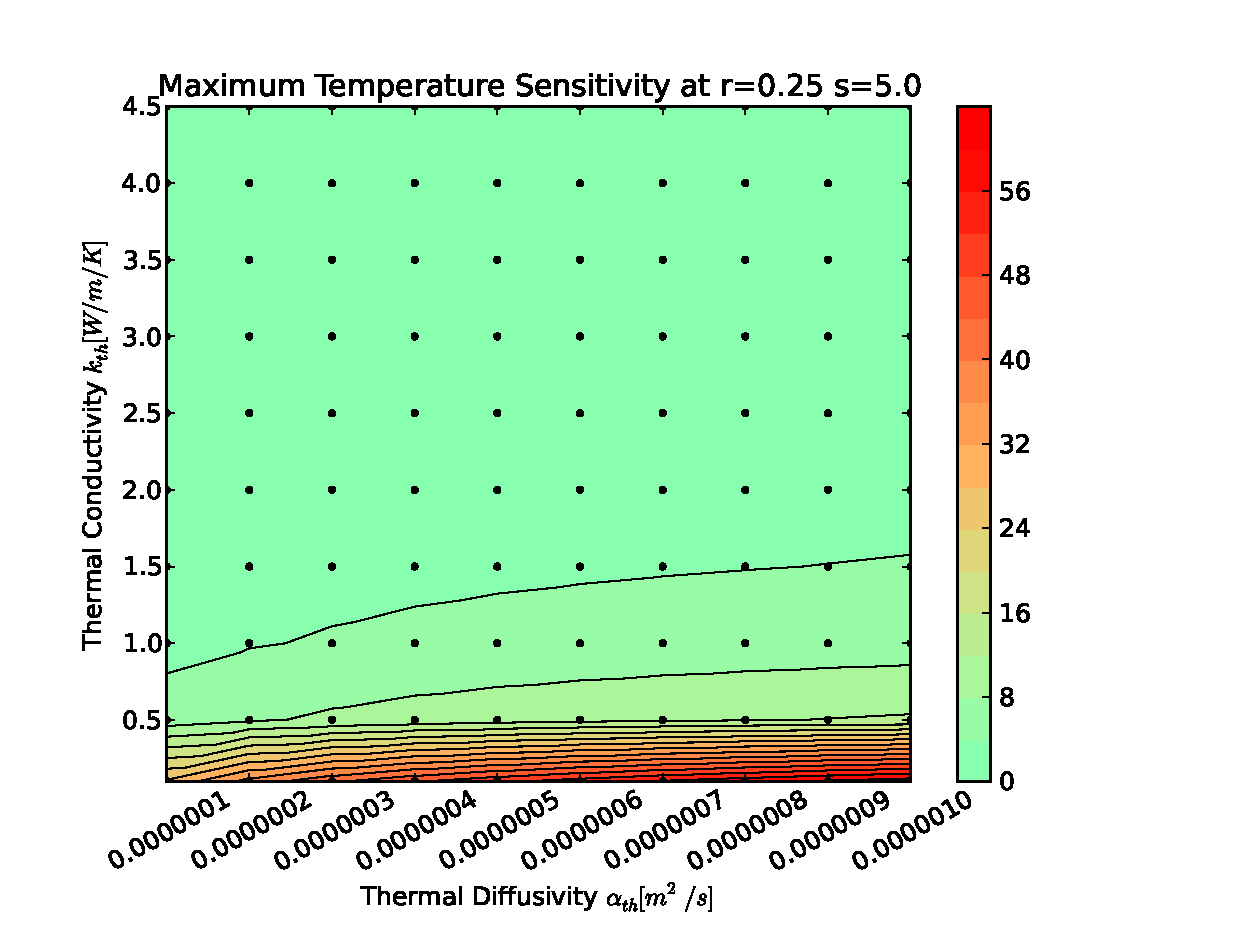
\includegraphics[height=0.7\textheight]{./thermal_demonstration/diffusivity/ak.eps}
%\caption[$\alpha_{th}$ vs. $K_{th}$ Sensitivity in Cyder]{Cyder trends agree 
%with those of the LLNL model, in which increased thermal diffusivity results in 
%decreased thermal depsoition in the near field. The above example thermal 
%profile results from 10kg of $^{242}Cm$.} 
%\label{fig:ar}
%\end{center}
%\end{figure}
%\end{frame}
%
%\begin{frame}[ctb!]
%\frametitle{Cyder Thermal Diffusivity and Limiting Radius Sensitivity}
%\begin{figure}[htbp!]
%\begin{center}
%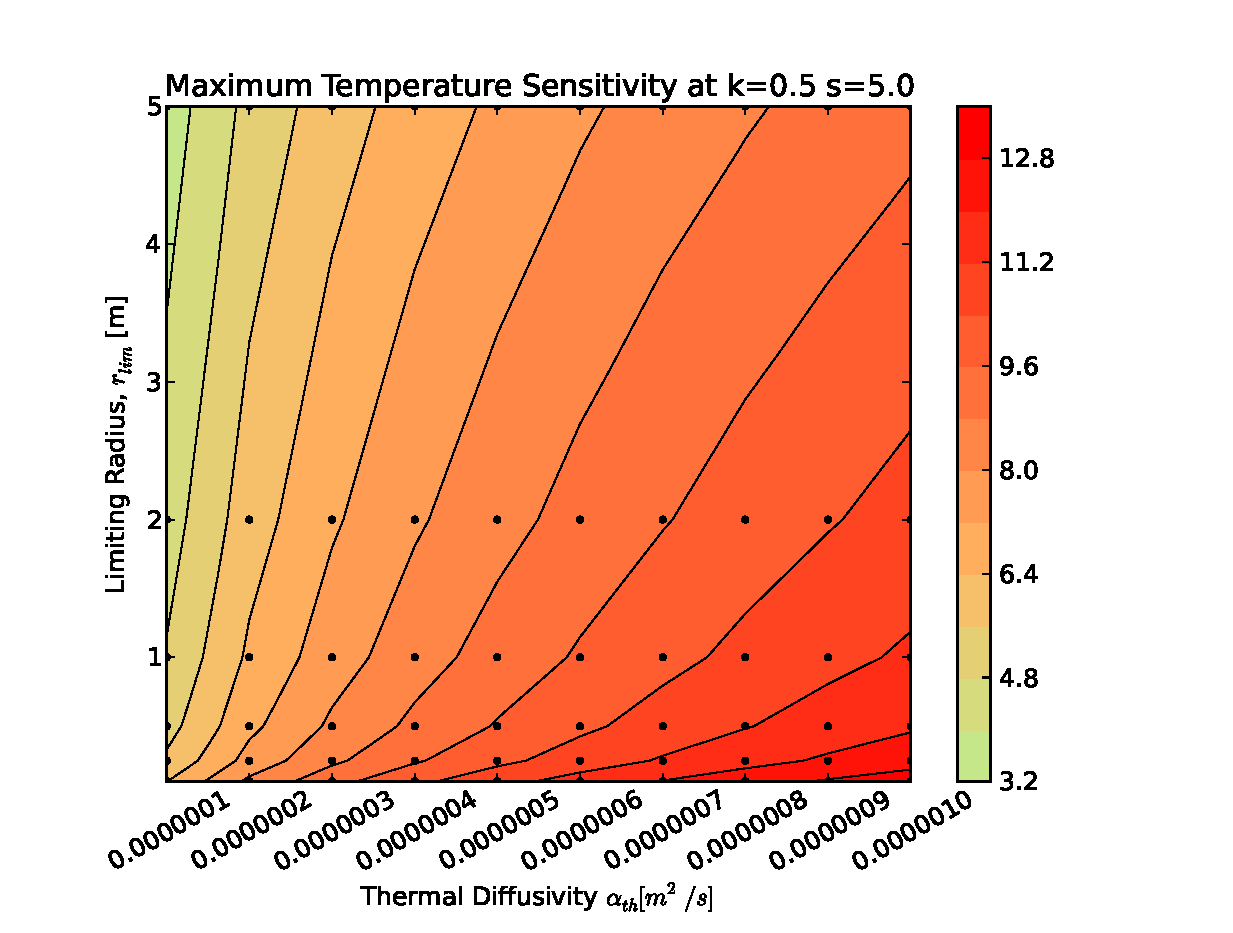
\includegraphics[height=0.7\textheight]{./thermal_demonstration/diffusivity/ar.eps}
%\end{center}
%\caption[$\alpha_{th}$ vs. $r_{lim}$ Sensitivity in Cyder]
%{Cyder trends agree with those of the LLNL model. The importance of the 
%limiting radius decreases with increased $K_{th}$. The above example thermal 
%profile results from 10kg of $^{242}Cm$.}
%\label{fig:ak}
%\end{figure}
%\end{frame}
%

\subsection{Waste Package Spacing Sensitivity Validation}\label{sec:spacing}
The waste package spacing, $s$ of geologic repository concept effects the areal 
decay heat burden in the repository and has a strong effect on the thermal 
energy deposited per unit area in the medium. 

\subsubsection{LLNL Model Results}

In the creation of the \gls{STC} database, the waste package spacing was varied 
across a number of values for each isotope, $i$, limiting 
radius $r_{calc}$, thermal diffusivity $\alpha_{th}$, and thermal conductivity $K_{th}$, considered.  By 
varying the waste package spacing of the geometric layout from $0.1-5 [m]$
this sensitivity analysis succeeds in capturing the domain of 
waste package spacings present in geologic repository concepts under 
consideration. 

\begin{figure}[htbp!]
\begin{center}
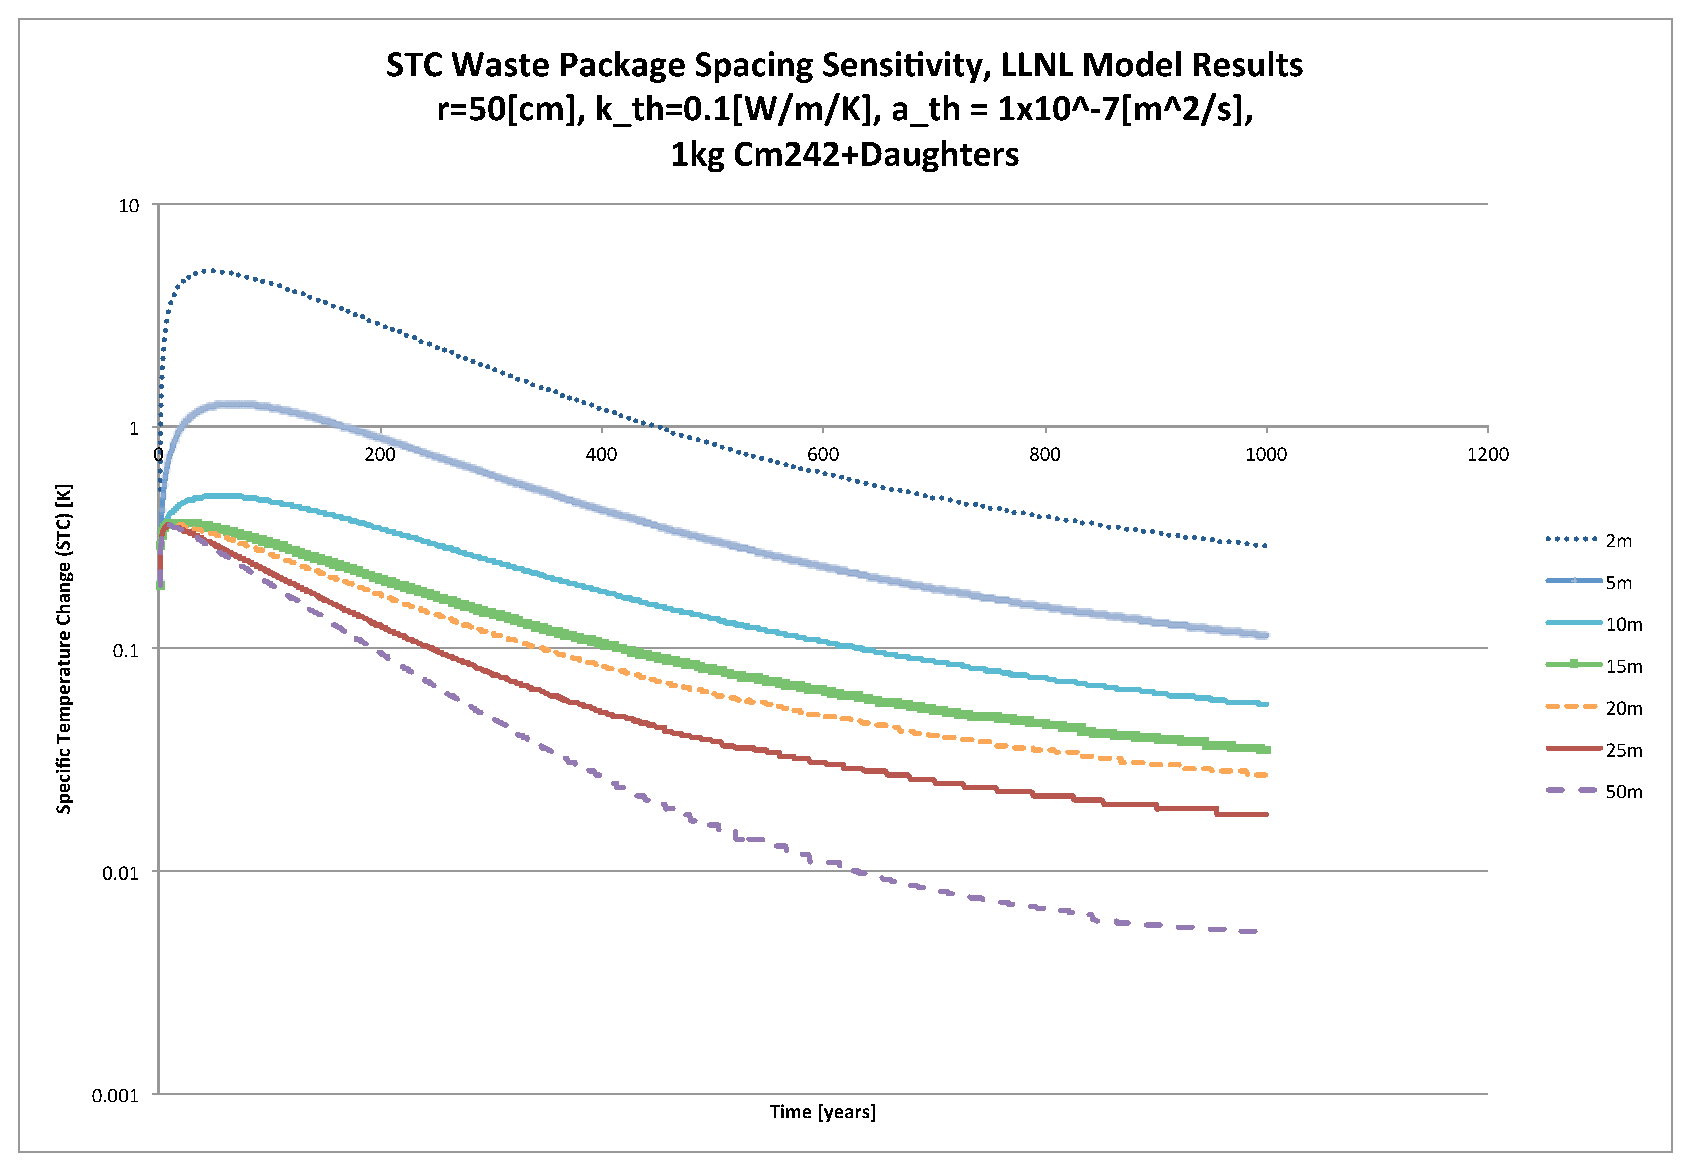
\includegraphics[width=\columnwidth]{./thermal_demonstration/spacing/Cm242spacing_sens.eps}
\end{center}
\caption[$K_{th}$ Sensitivity to $s$]{Increased waste package 
spacing decreases areal thermal energy deposition 
(here represented by \gls{STC}) in the near field (here $r_{calc} = 0.5m$).}
\label{fig:Cm242spacing_sens}
\end{figure}

Figure \ref{fig:Cm242spacing_sens} shows the trend in which increased waste package spacing of a medium decreases areal thermal energy 
deposition in the near field. This indicates that waste package spacing is 
an important parameter for repository concept design.

Similarly, the location of the limiting radius has a strong effect on the 
waste package loading limit, for a fixed limiting temperature. In Figure 
\ref{fig:Cm242r_lim_sens}, the trend is demonstrated in which increased limiting 
radius decreases the thermal energy contributing to the thermal limit. 


\begin{figure}[htbp!]
\begin{center}
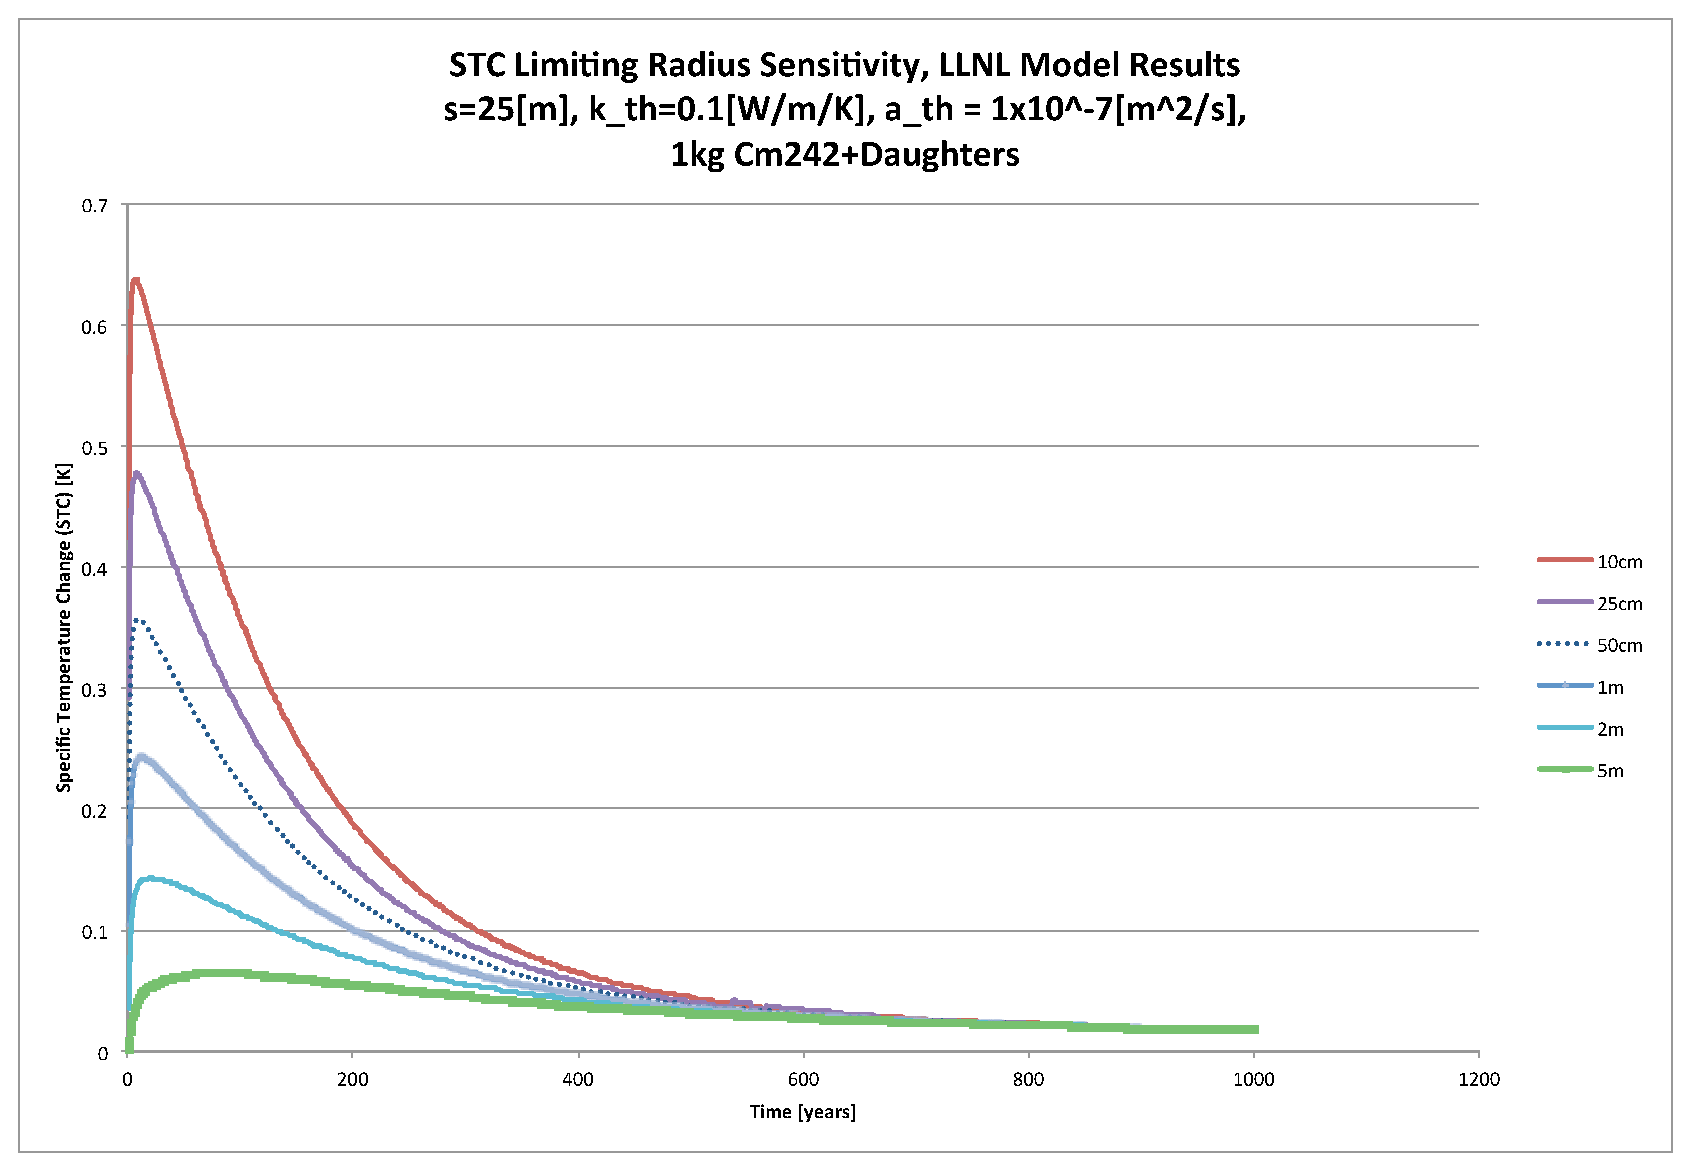
\includegraphics[width=\columnwidth]{./thermal_demonstration/spacing/Cm242r_lim_sens.eps}
\end{center}
\caption[$K_{th}$ Sensitivity to $r_{lim}$]{Increased limiting radius 
decreases thermal energy deposition contributing to the thermal limit
(here represented by \gls{STC}).}
\label{fig:Cm242r_lim_sens}
\end{figure}


\subsubsection{Cyder Results}

In a similar analysis, the thermal diffusivity was compared both with the 
spacing between waste packages and the limiting radius. 

Figure \ref{fig:rs} validates the trend noted above that 
increased waste package spacing in a repository concept decreases areal thermal energy deposition 
in the near field.  Additionally, analysis with the \Cyder STC database 
demonstrates the way in which the importance of $r_{lim}$, the limiting radius, 
impacts the maximum calculated temperature at that radius. 


\begin{figure}[htbp!]
\begin{center}
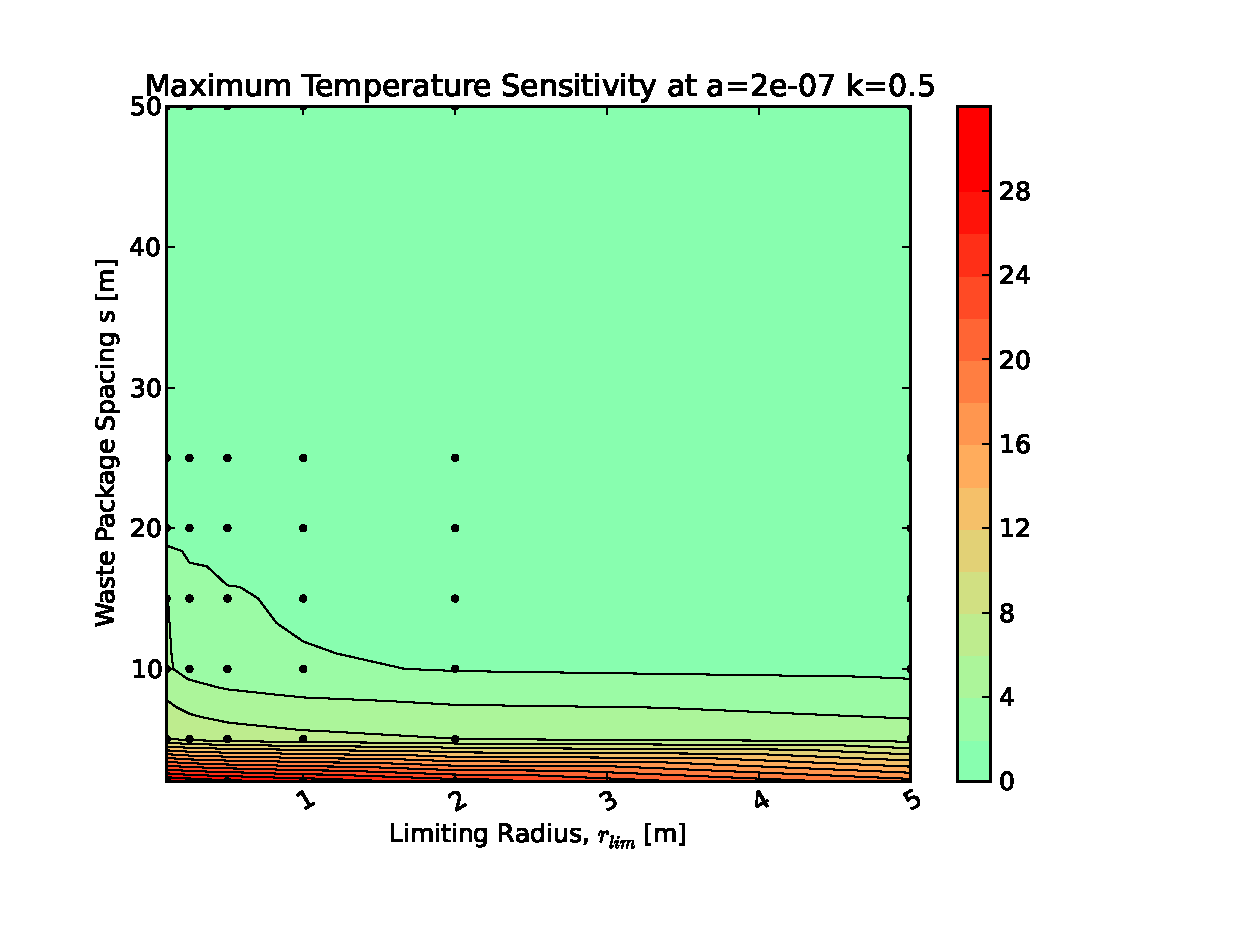
\includegraphics[width=\columnwidth]{./thermal_demonstration/spacing/rs.eps}
\end{center}
\caption[$\alpha_{th}$ vs. $r_{lim}$ Sensitivity in Cyder]
{Cyder results agree with 
those of the LLNL model. The importance of the limiting radius decreases with 
increased $K_{th}$. The above example thermal profile results from 10kg of 
$^{242}Cm$}
\label{fig:rs}
\end{figure}






\begin{frame}[ctb!]
  \frametitle{lp}
  
\begin{frame}[ctb!]
\begin{figure}[ht]
\centering
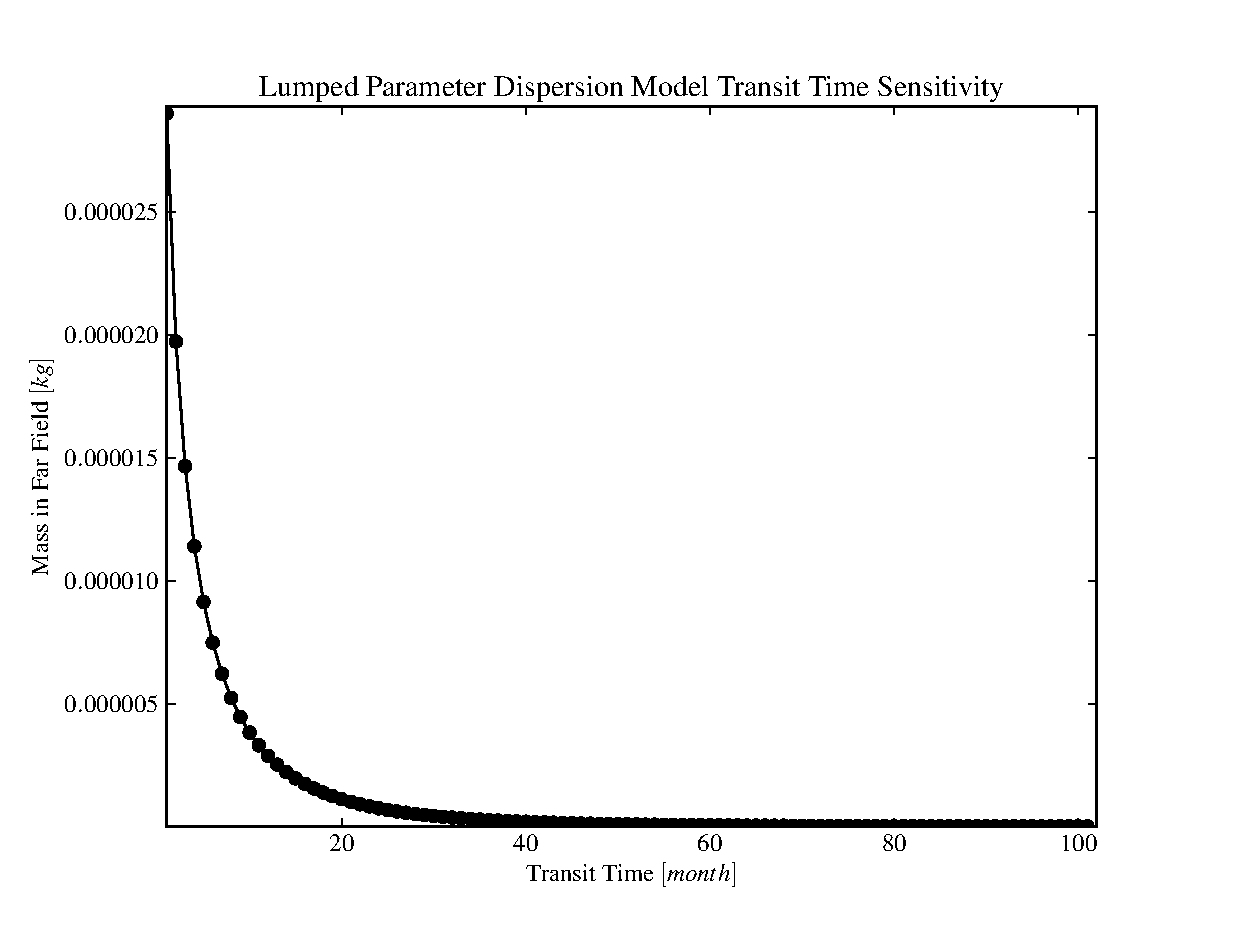
\includegraphics[width=0.8\textwidth]{./chapters/demonstration/base/lpDM_t_t.eps}
\caption[Lumped Parameter Dispersion Model Transit Time Sensitivity]{The transit time 
parameterization of the lumped parameter dispersion model of radionuclide 
transport has a strong effect on the material reaching the far field after 30 
years.  }
\label{fig:lp_t_t_begin}
\end{figure}
\end{frame}

\begin{frame}[ctb!]
\begin{figure}[ht]
\centering
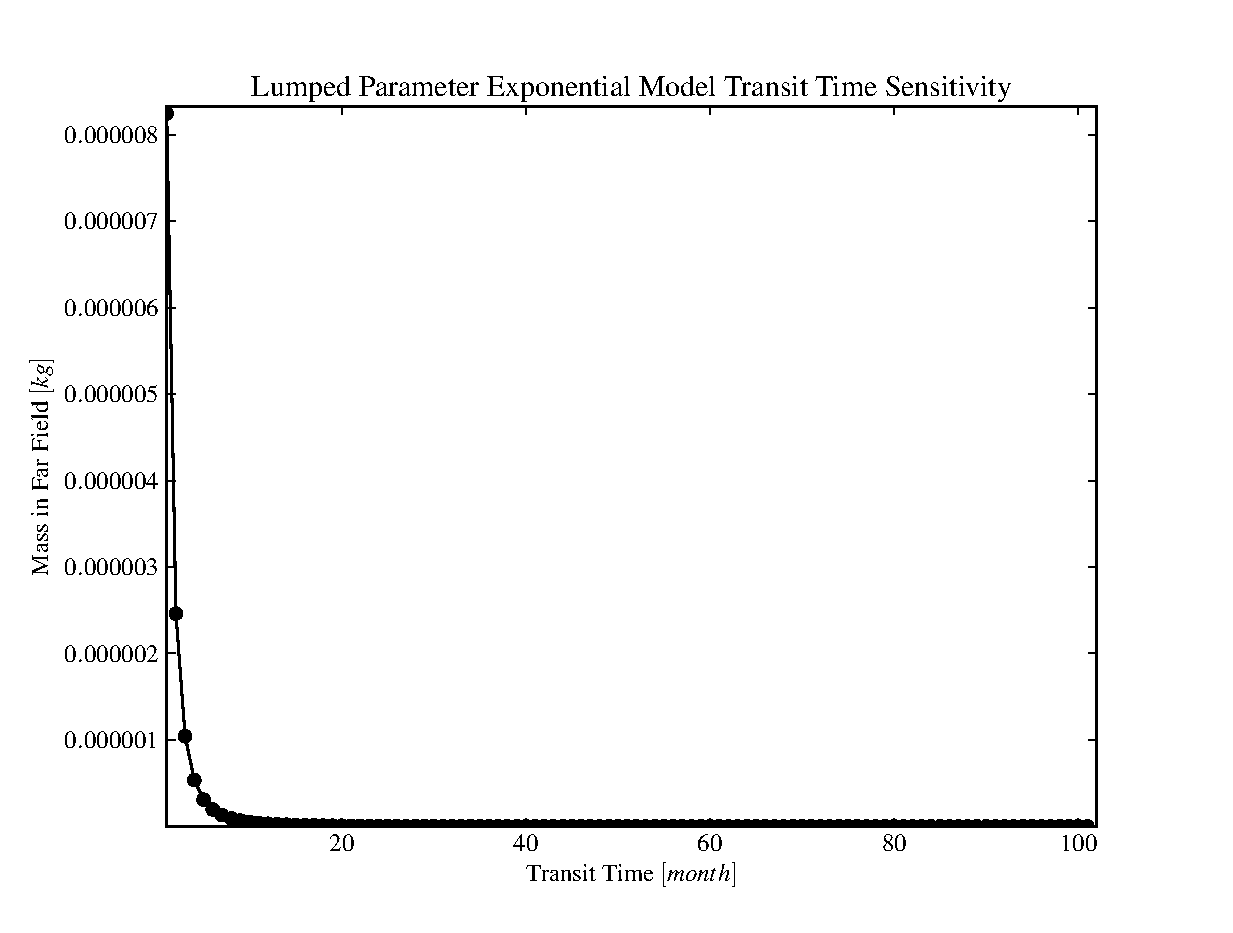
\includegraphics[width=0.8\textwidth]{./chapters/demonstration/base/lpEXPM_t_t.eps}
\caption[Lumped Parameter Exponential Model Transit Time Sensitivity]{The transit time 
parameterization of the lumped parameter exponential model of radionuclide 
transport has a strong effect on the material reaching the far field after 30 
years.  }
\end{figure}
\end{frame}

\begin{frame}[ctb!]
\begin{figure}[ht]
\centering
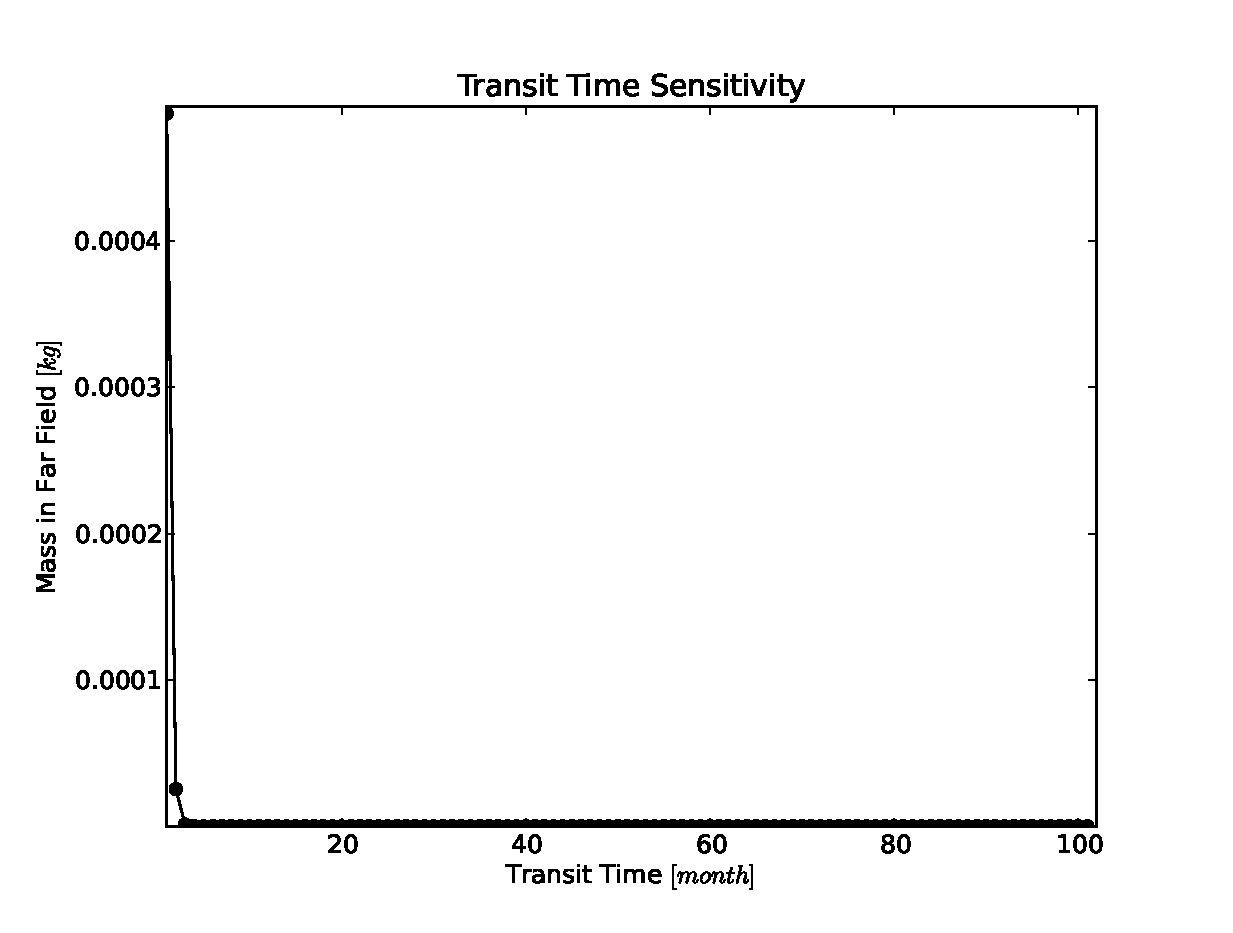
\includegraphics[width=0.8\textwidth]{./chapters/demonstration/base/lpPFM_t_t.eps}
\caption[Lumped Parameter Piston Flow Model Transit Time Sensitivity]{The transit time 
parameterization of the lumped parameter piston flow model of radionuclide 
transport has a strong effect on the material reaching the far field after 30 
years.  }
\label{fig:lp_t_t_end}
\end{figure}
\end{frame}

  \end{minipage}
\end{frame}

%%%%%%%%%%%%%%%%%%%%%%%%%%%%%%%%%%%%%%%%%%%%%%%%%%%%%%%%%%%%%%%%%%%%%%%%%%%%%%%%
\bibliographystyle{ans}
\bibliography{global_paper.bib}
\end{document}


